

شبکه عصبی زیر را در نظر بگیرید.  در این شبکه، گره‌های تک‌دایره‌ای نشان‌دهنده متغیرها (به عنوان مثال $x_1$ متغیر ورودی، $h_1$ متغیر میانی و $\hat{y}$ متغیر خروجی است.) و گره‌های دودایره‌ای نشان‌دهنده توابع هستند.

\begin{figure}[H]
\centering 
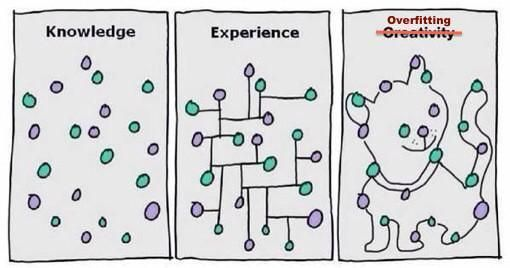
\includegraphics[width=0.7\textwidth]{questions/image.png}
\end{figure}


فرض کنید تابع هزینه $L_2$ به صورت $L(y, \hat{y})=||y-\hat{y}||^2_2$ تعریف شده است. اگر یک داده با مقدار $(x_1,x_2,x_3,x_4)=(1,2,-1,0)$ و برچسب واقعی $1$ داشته باشیم، از الگوریتم  $backpropagation$ برای محاسبه مشتق جزئی $L$ نسبت به $w_1$ استفاده کنید.

\begin{center}
    $f(x) = ReLU(x) - 2 ReLU(x-1) + 0.5ReLU(x+1)$\\
    $(w_1, w_2, w_3, w_4, w_5, w_6) = (1, -0.25, 0, 1, 2, -1)$
\end{center}